% Author: Izaak Neutelings (January 2021)
\documentclass[border=3pt,tikz]{standalone}
\usepackage{tikz}
\tikzset{>=latex} % for LaTeX arrow head

\begin{document}


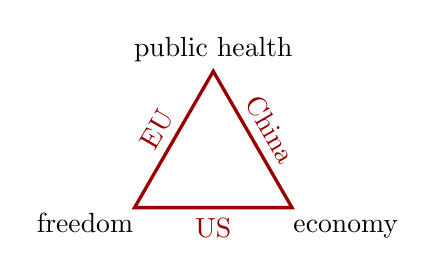
\begin{tikzpicture}
  \def\L{2}
  \coordinate (T)  at (0,{\L*sin(60)});
  \coordinate (L)  at (-\L/2,0);
  \coordinate (R)  at ( \L/2,0);
  \draw[very thick,red!60!black]
    (T) -- (L) node[midway,above,rotate=60] {EU}
        -- (R) node[midway,below] {US}
        -- cycle node[midway,above,rotate=-60] {China};
  \node[above] at (T) {public health};
  \node[below left=-3] at (L) {\strut freedom};
  \node[below right=-3] at (R) {\strut economy};
\end{tikzpicture}

% RADAR CHART
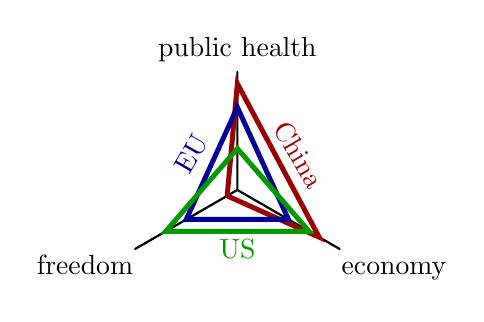
\begin{tikzpicture}
  \def\L{1.5}
  \coordinate (O)  at (0,0);
  \coordinate (T)  at (90:\L);
  \coordinate (R)  at (-30:\L);
  \coordinate (L)  at (-150:\L);
  \draw[thick,line cap=round]
    (O) -- (T) node[above] {public health}
    (O) -- (R) node[below right=-3] {\strut economy}
    (O) -- (L) node[below left=-3] {\strut freedom};
  %\draw[very thick,red!60!black,line cap=round] % China
  %  (90:0.9*\L) -- (-30:0.8*\L)
  %  (-30:0.8*\L) -- (-150:0.1*\L)
  %  (-150:0.1*\L) -- (90:0.9*\L);
  \draw[line width=1.8,red!60!black] % China
    (90:0.9*\L) -- (-30:0.8*\L) -- (-150:0.1*\L) -- cycle;
  \draw[line width=1.8,blue!60!black] % EU
    (90:0.7*\L) -- (-30:0.5*\L) -- (-150:0.5*\L) -- cycle;
  \draw[line width=1.8,green!60!black] % US
    (90:0.35*\L) -- (-30:0.7*\L) -- (-150:0.7*\L) -- cycle;
  \node[red!60!black,rotate=-60] at (30:0.6*\L) {China};
  \node[blue!60!black,rotate=60] at (142:0.5*\L) {EU};
  \node[green!60!black] at (-90:0.5*\L) {US};
\end{tikzpicture}

\end{document}